\documentclass[]{article}
\usepackage{lmodern}
\usepackage{amssymb,amsmath}
\usepackage{ifxetex,ifluatex}
\usepackage{fixltx2e} % provides \textsubscript
\ifnum 0\ifxetex 1\fi\ifluatex 1\fi=0 % if pdftex
  \usepackage[T1]{fontenc}
  \usepackage[utf8]{inputenc}
\else % if luatex or xelatex
  \ifxetex
    \usepackage{mathspec}
  \else
    \usepackage{fontspec}
  \fi
  \defaultfontfeatures{Ligatures=TeX,Scale=MatchLowercase}
\fi
% use upquote if available, for straight quotes in verbatim environments
\IfFileExists{upquote.sty}{\usepackage{upquote}}{}
% use microtype if available
\IfFileExists{microtype.sty}{%
\usepackage{microtype}
\UseMicrotypeSet[protrusion]{basicmath} % disable protrusion for tt fonts
}{}
\usepackage[margin=1in]{geometry}
\usepackage{hyperref}
\hypersetup{unicode=true,
            pdftitle={Homework 1},
            pdfborder={0 0 0},
            breaklinks=true}
\urlstyle{same}  % don't use monospace font for urls
\usepackage{graphicx,grffile}
\makeatletter
\def\maxwidth{\ifdim\Gin@nat@width>\linewidth\linewidth\else\Gin@nat@width\fi}
\def\maxheight{\ifdim\Gin@nat@height>\textheight\textheight\else\Gin@nat@height\fi}
\makeatother
% Scale images if necessary, so that they will not overflow the page
% margins by default, and it is still possible to overwrite the defaults
% using explicit options in \includegraphics[width, height, ...]{}
\setkeys{Gin}{width=\maxwidth,height=\maxheight,keepaspectratio}
\IfFileExists{parskip.sty}{%
\usepackage{parskip}
}{% else
\setlength{\parindent}{0pt}
\setlength{\parskip}{6pt plus 2pt minus 1pt}
}
\setlength{\emergencystretch}{3em}  % prevent overfull lines
\providecommand{\tightlist}{%
  \setlength{\itemsep}{0pt}\setlength{\parskip}{0pt}}
\setcounter{secnumdepth}{0}
% Redefines (sub)paragraphs to behave more like sections
\ifx\paragraph\undefined\else
\let\oldparagraph\paragraph
\renewcommand{\paragraph}[1]{\oldparagraph{#1}\mbox{}}
\fi
\ifx\subparagraph\undefined\else
\let\oldsubparagraph\subparagraph
\renewcommand{\subparagraph}[1]{\oldsubparagraph{#1}\mbox{}}
\fi

%%% Use protect on footnotes to avoid problems with footnotes in titles
\let\rmarkdownfootnote\footnote%
\def\footnote{\protect\rmarkdownfootnote}

%%% Change title format to be more compact
\usepackage{titling}

% Create subtitle command for use in maketitle
\newcommand{\subtitle}[1]{
  \posttitle{
    \begin{center}\large#1\end{center}
    }
}

\setlength{\droptitle}{-2em}

  \title{Homework 1}
    \pretitle{\vspace{\droptitle}\centering\huge}
  \posttitle{\par}
    \author{}
    \preauthor{}\postauthor{}
    \date{}
    \predate{}\postdate{}
  

\begin{document}
\maketitle

\section{Exercise 1}\label{exercise-1}

\subsection{Problem}\label{problem}

An Austin real-estate developer is interested in the possible economic
impact of ``going green'' in her latest project: a new 15-story (height)
mixed-use (not all green, nor all non-green) building on East Cesar
Chavez (location), just across I-35 from downtown. 250,000 square feet
(size) expected baseline construction costs are \$100 million (different
types of rental rate) earning rents for 30 years or more (possible
building age)

\section{Question 1}\label{question-1}

I do not agree with the analysis given. If we look at the distribution
of rent according to the size of the properties, we observe that the
median rate may not vary that much. However, if we seperate the rent
based on the type of contract, either gross contract or net contract,
there will be discrepancies across median rental rate based on property
size. I will classify the size of property based on four quartiles based
on the collecting data.

\begin{verbatim}
##    Min. 1st Qu.  Median    Mean 3rd Qu.    Max. 
##    1624   50891  128838  234638  294212 3781045
\end{verbatim}

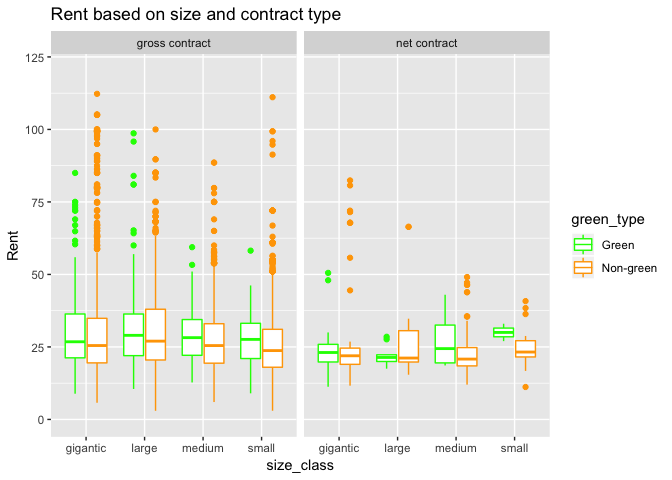
\includegraphics{Homework1_files/figure-latex/unnamed-chunk-2-1.pdf}

As you can observe from the box plot, the medians rental rate between
green versus non-green property for large properties
(\(128838 <x< 294212 \ {feet^{2}}\)) do not differ much in net contracts
but vary greatly in gross contracts, with green building enjoys around
\$3.20. Hence, the rough estimate of difference in rental rate between
green and non-green building is questionable.

The next questionable assumption is the rent will be constant throughout
the life of the building. I will look into the median rent for an
interval of every 10 years

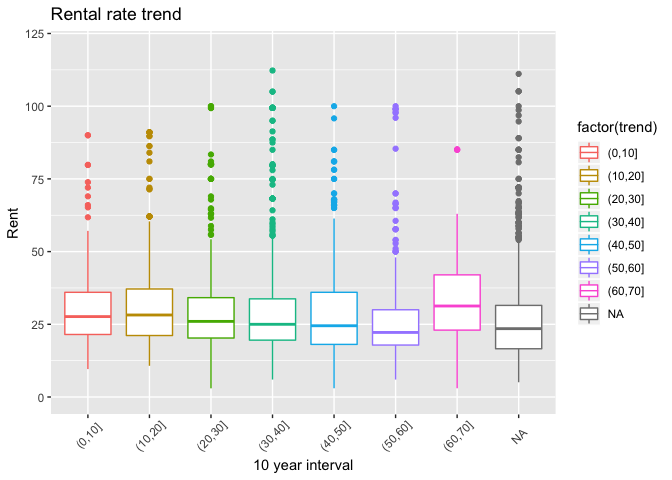
\includegraphics{Homework1_files/figure-latex/unnamed-chunk-3-1.pdf}

Hence, forecasting the rent to stay constant throughout building's
lifetime is irrelevant. Therefore, the revenue stream will not be
constant, making the profit prediction after cost repcuperation is
dubious.


\end{document}
